\section{Circuit série et intensité (4 points)}

\begin{questions}
	\question Trace le schéma normalisé du circuit ci-dessous. Repère les intensités $I_1$ à $I_4$ qui sont mesurées par les ampèremètres $A_1$ à $A_4$.
	\begin{solution}
		\begin{center}
			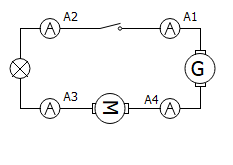
\includegraphics[scale=1.1]{img/ex4_exam}
		\end{center}
	\end{solution}
	
	
	\question L'ampèremètre $A_3$ mesure une intensité $I_3$ de \num{0.250} A. Que valent $I_1$, $I_2$ et $I_4$.
	\begin{solution}
		C'est un circuit série, donc l'intensité du courant est la même partout, on a donc $I_1 = I_2 =I_4 = \num{0.250} A$
	\end{solution}
\end{questions}

\begin{center}
	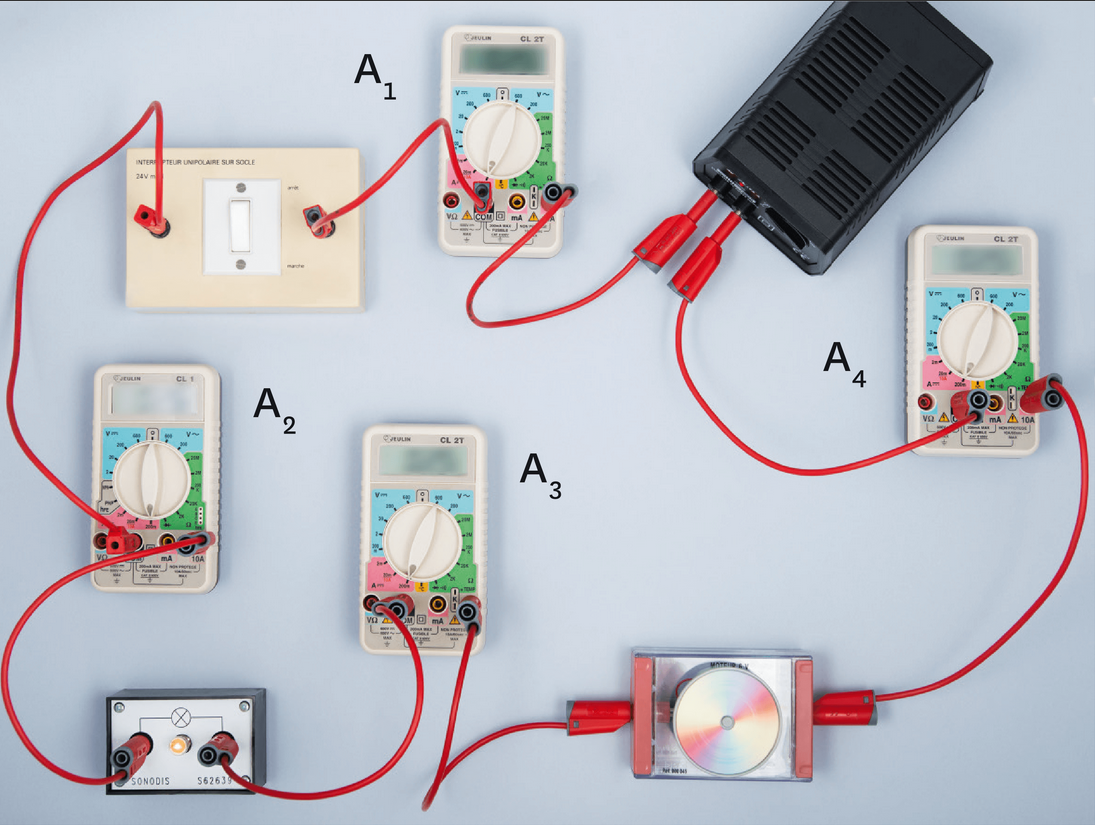
\includegraphics[scale=0.4]{img/ex15}
\end{center}